\documentclass[11pt]{article}

\usepackage[empty]{fullpage}
\usepackage{tabularx}               % For table
\usepackage[english]{babel}
\usepackage{amsmath}                                % For textit, textbf, etc
\usepackage{graphicx}                               % For includegraphics
\usepackage{wrapfig}                                % For wrapfig environment
\usepackage{paralist}                               % For compactitem 
\usepackage[dvipdfm]{hyperref}                               % For links
\usepackage{xcolor}                                 % For colors
\usepackage{romannum}                               % For roman numbers
\usepackage{ifthen}                                 % Required for ifthenelse statements
%\usepackage{geometry}                % Already loaded by graphicx

\pagestyle{empty}                                   % No pagenumbers/headers/footers

%%% Custom sectioning (sectsty package)
\usepackage{sectsty}
\sectionfont{%                                  % Change font of \section command
  \usefont{OT1}{phv}{m}{n}%                   
  \sectionrule{0pt}{0pt}{-10pt}{1pt}
}
\subsectionfont{%                             % Change font of \subsection command
  \usefont{OT1}{phv}{m}{n}%                   
  %\sectionrule{0pt}{0pt}{-10pt}{1pt}
}

%%% Macros

\newcommand{\sepspace}{\vspace*{1em}}           % Vertical space macro
\newcommand{\NewPart}[1]{\section*{\uppercase{#1}}}
\newcommand{\NewSubPart}[1]{\subsection*{#1}}

\newcommand{\MyName}[1]{
    \noindent
  \Huge \usefont{OT1}{phv}{m}{n} #1 \hfill        % Name
  \par \normalsize \normalfont
}

\newcommand{\SimpleEntry}[1]{
  \noindent\hangindent=0.5cm\hangafter=0          % Indentation
  #1 \par                                         % Entry 
}

% Earlier I did this, but now I have used a table as it is more compact
\newcommand{\Education}[4]{                    % Takes 4 variables
    %\noindent\hangindent=0.5cm\hangafter=0          % Indentation
  \begin{itemize}
    \item\textbf{#1}                                     % School College
    \hfill\textit{#2}\\                           % Time
    \text{#3}\\                                       % What, degree
    \textit{#4}                               % Average, Focus, etc
    \normalsize \par
  \end{itemize}
}

\newcommand{\TitleEntry}[2]{                     
  \noindent\hangindent=0.5cm\hangafter=0            % Indentation
  \parbox{3cm}{                                   % Box to align text
      \textit{#1}
  }                                         % Title
  #2 \par                                         % Entry 
}

% NOTE : textit{} takes newline if the text is full
% Parameters : Name of project, year, mentor, Description and link
\newcommand{\Project}[5]{                           % Takes 5 parameters
    %\noindent\hangindent=0.5cm\hangafter=0          % Indentation
  \begin{itemize}
    \item\textbf{#1}                                     
      \hfill\textbf{#2}\\                     
    \text{#3}\\
    \textit{#4}                                     
    \hfill\textit{\textcolor{blue}{\href{#5}{Link}}}                               
    \normalsize \par
  \end{itemize}
}

\newcommand{\WorkExp}[4]{                           % Takes 4 parameters
    %\noindent\hangindent=0.5cm\hangafter=0         % That takes Internship Name                                                         % Date, Description, Link
  \begin{itemize}
    \item\textbf{#1}                                     
      \hfill\textbf{#2}\\                     
    \textit{#3}                                     
    \hfill\textit{\textcolor{blue}{\href{#4}{Link}}}                               
    \normalsize \par
  \end{itemize}
}

\newcommand{\Skill}[3]{
    %\noindent\hangindent=0.5cm\hangafter=0          % Indentation
  \begin{itemize}
    \item\textbf{#1}\\                                   % Topic of skill
    \textit{#2}                                     % Description of Skill
    \ifthenelse{\equal{#3}{}}
        {}                                                        % if true then {}
        { \hfill\textit{\textcolor{blue}{\href{#3}{Link}}} }       % else this
    \normalsize \par
  \end{itemize}
}

\newcommand{\Training}[3]{
     \noindent\hangindent=0.5cm\hangafter=0          % Indentation
  \textbf{#1}                                  % Description of Training
  \hfill\textbf{#2}\\                           % Date of Training
    \textit{#3}
    \normalsize \par
}

\newcommand{\Achievement}[3]{
    %\noindent\hangindent=0.5cm\hangafter=0          % Indentation
  \begin{itemize}
    \item\textbf{#1}\\                                   % Topic of Achievement
    \textit{#2}                                     % Description of Achievement
    \ifthenelse{\equal{#3}{}}
        {}                                                        % if true then {}
        { \hfill\textit{\textcolor{blue}{\href{#3}{Link}}} }       % else this
    \normalsize \par
  \end{itemize}
}

\newcommand{\Activity}[2]{
     %\noindent\hangindent=0.5cm\hangafter=0          % Indentation
  \begin{itemize}
    \item\textbf{#1}\\                               % Topic of Activity
    \textit{#2}                                    % Description of Activity
      \normalsize \par
  \end{itemize}
}


%%% Begin Document
\begin{document}
\begin{wrapfigure}{l}{1cm}
    \vspace*{0.75cm}
	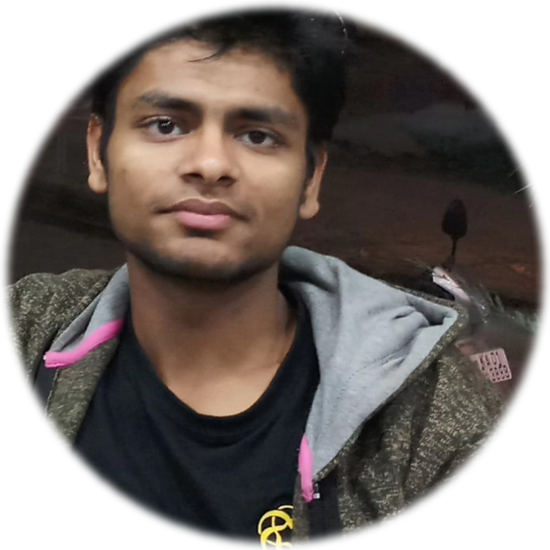
\includegraphics[width=0.13\textwidth,natwidth=200,natheight=200]{transparent.png}
	\hspace*{\fill}
	\vspace{-1.5cm}
\end{wrapfigure}



\hfill\MyName{Vaibhav Jindal}

\sepspace

%%% Personal details
%\NewPart{Personal details}
    
\hfill\SimpleEntry{Male, 21}
\hfill\SimpleEntry{+91 9410833183}
\hfill\SimpleEntry{vaibhavjindal1999@gmail.com}
\hfill\SimpleEntry{Ghaziabad, Uttar Pradesh}
\hfill\SimpleEntry{\textcolor{blue}{\href{https://www.linkedin.com/in/vaibhav-jindal-818060164}{LinkedIn}}}


%%% Carrer Objective
\NewPart{Carrer Objective}
\SimpleEntry{\large A self-motivated and an inspired techie, who is looking for great opportunities and growth. Always eager to learn something new. Intrigued and inclined towards areas of Machine Learning, Deep Learning and Reinforcement Learning.}


%%% Education
\NewPart{Education}
\setlength{\tabcolsep}{4pt} 	% Default value: 6pt
\small{\begin{tabularx}
{\dimexpr\textwidth-4mm\relax\setlength\extrarowheight{2pt}}{|c|c|c|c|}
  \hline
  \textbf{Degree/Certificate } & \textbf{Institute/Board} & \textbf{CGPA/Percentage} & \textbf{Year}\\
  \hline
  B.Tech. & Indian Institute of Technology, Palakkad & 8.19 (Current) & 2017-Present\\
  \hline
  Class \Romannum{12} & CBSE Board & 91\% & 2016 \\
  \hline
  Class \Romannum{10} & CBSE Board & 91\% & 2014 \\
  \hline
\end{tabularx}}
\vspace{-2mm}
\sepspace


%%% Elective Courses
%\NewPart{Elective Courses}
%\text{Machine Learning}
%\hfill{Theory of Computation}\\
%\text{Reinforcement Learning}
%\hfill{Algebra}

%%% Projects
\NewPart{Projects}
\Project{Face Detection Algorithm}
{Jun 2018 to Sep 2018}
{Data Analysis Club at IITPKD}
{We made a face detection algorithm using HOG descriptor to detect faces in photos. It makes a bounding box around the face of people.We trained the model on 10K photos of people from Caltech Webfaces Dataset}
{https://drive.google.com/drive/folders/1tKLkB-zteWIj81nOL6JcBzZDrD-C5IAm?usp=sharing}

\Project{Online E-Challan system}
{Dec 2017 to Mar 2018}
{Sumesh KS (sumesh@iitpkd.ac.in)}
{E-Challan system for both police and public.Police send the violation details to defaulter and public will be able to deposit the fine amount within the due date}
{http://iit.pscquestion.in}


%%% Technical Skills
%% Links are also included in skills
\NewPart{Technical Skills}
\Skill{Competitive Programming}
{I have a fair knowledge of Data Structures and Algorithms. \\Username on Codechef, UVA : vjac, Hackerrank : vaibhav\_jindal}
{https://www.codechef.com/users/vjac} 

\Skill{Hardware and assembly language}
{Verilog and Mips from the courses offered in Computer Organisation and Digital Systems}
{}                                                      % last argument is empty

\Skill{Programming Languages}
{C++ (Moderate), C (Moderate), Python3 (Moderate), Java (Begineer)}
{}                                                      % last argument is empty

\Skill{Deep Learning Frameworks}
{Tensorflow, Keras, Pytorch: Learnt from Deep\_Learning course from Coursera}
{https://www.coursera.org/account/accomplishments/specialization/828BASVWCMAT}


%%% Training and Workshop
\NewPart{Training and Workshop}
\Training{Workshop on IOT in banglore at Lemma Labs,Alumni IIT Madras}
{Jan 2018}


%%% Position of Responsibility
\NewPart{Position of Responsibility}
\begin{itemize}
	\item \SimpleEntry{Career Development Cell Coordinator (2020 -present)}
	\item\SimpleEntry{Class Representative (2020 Winter)}
	\item\SimpleEntry{Mentor at Data Analysis Club at IIT Palakkad (2018 - 2019)}
	\item\SimpleEntry{Class Representative (2017 Summer)}
\end{itemize}

%%% Achievements
%% Links are included as third argument
\NewPart{Achievements}
\Achievement{Star Clustering Identification at Inter IIT Tech Meet 2018}
{Involve data analysis and inference from dataset for a globular star cluster. Task is using the datasets appropriately to analyze the globular cluster to determine some parameters and peculiarities of the same}
{}

\Achievement{PlutoX at Inter IIT Tech Meet 2018 }
{The PlutoX is programmed using a development environment, the Cygnus IDE. The programming itself is done in C++ with PlutoX API library. We implemented several movements, flip-flops and in built sensors in the PlutoX}
{}

\Achievement{Google Code Jam 2019}
{Participated in Round 1C}
{}

\Achievement{CodeChef Snackdown 2019}
{Participated in Pre-Elemination Round}
{}

\Achievement{Participated in Smart India Hackathon 2017}
{Our problem statement was to build an user interface for E-Challan system. We made a Website for both common people and police officers. We made a database and a system to send details to the defaulter of their offence}
{}


%%% Extra Curricular Activities
\NewPart{Extra Curricular Activities}
\Activity{Badminton Player}
{Went for the trials for inter IIT Sports meet. Participated in inter branch sports competition in badminton}
\end{document}

